\documentclass[aspectratio=43,scheme=plain]{ctexbeamer}
%\mode<presentation>
\setcounter{tocdepth}{2}

%\usepackage{xeCJK}
\setCJKmainfont{IPAexGothic}

%\usetheme{Antibes}
%\setbeamertemplate{navigation symbols}{}
%\setbeamertemplate{caption}[numbered]
%\usecolortheme{owl}

\usetheme{trigon}
\trigonset{titlestyle=style2,
	sectionpage=none,
	headingcolor=theme,
	numbering=fraction,
	block=fill
}


%\usetheme[nofirafonts,numbering=progressbar,totalframenumbering=yes]{focus}

%\usetheme[showmaxslides,customfont,nofooter,darkmode]{pureminimalistic}
%\renewcommand{\logotitle}{}
%\renewcommand{\logoheader}{}
%\renewcommand{\logofooter}{}

%\usetheme[numbering=fraction,progressbar=frametitle,sectionpage=none,block=fill,subsectionpage=none]{metropolis}

\usepackage{pgfpages}
%\pgfpagesuselayout{4 on 1}[a4paper,landscape]
%\setbeameroption{show notes on second screen}


\AtBeginSection[]{
	\begin{frame}{Contents}
		\tableofcontents[currentsection]
\end{frame}}

\AtBeginSubsection[]{
	\begin{frame}{Contents}
		\tableofcontents[currentsection,currentsubsection]
\end{frame}}
\usefonttheme{professionalfonts}

\usepackage{siunitx}
\usepackage[version=4]{mhchem}
\usepackage{amsmath}
\usepackage{amssymb}
\usepackage{amsfonts}
\usepackage{metalogo}
\usepackage{appendix}
\usepackage{xcolor}
%\pagecolor[RGB]{46,46,46}
%\color[RGB]{248,248,248}
\usepackage{framed}
\usepackage{tabularx}
\usepackage{colortbl}
\usepackage{enumerate}
\usepackage{wrapfig2}
\usepackage{graphicx}
\usepackage{subfigure} 
\usepackage{float} 
\usepackage{tikz}
\usepackage{qrcode}
\usepackage{booktabs}
\usepackage{multirow}

\renewcommand{\appendixtocname}{付録}
\renewcommand{\appendixpagename}{付録}
\renewcommand{\contentsname}{目次}
\renewcommand{\figurename}{Fig.}

\usepackage[hyperref=true,backend=biber,url=false,doi=false,dateabbrev=true,backref=false,maxnames=2,isbn=false]{biblatex}
\DeclareFieldFormat{biblabeldate}{\mkbibparens{\mkbibbold{#1}}}
\DeclareFieldFormat[article,periodical]{volume}{\mkbibbold{#1}}
\renewbibmacro{in:}{}
\addbibresource{reference.bib}%导入bib文件。

%\usepackage{hyperref}
\hypersetup{
	bookmarksnumbered=true,
	colorlinks=false,
	linkcolor=black,
	urlcolor=blue,
	citecolor=black,
	pdfauthor={B4},
	pdfcreator={XYX},
	pdftitle={Machine time report},
	pdfsubject={Galvano, },
	pdfkeywords={Exercise experiments}
}

\title{練習実験報告}
\author{肖宇笑}
\date{\today}
\definecolor{trigon}{RGB}{0,112,127}
\begin{document}
%	\maketitle 						   %for Metropolis, Antibes, focus
	\titleframe						    %for Trigon
	\begin{frame}[containsverbatim]{Is this the latest?}	
Click \textcolor{blue}{\href{https://github.com/xiaoyuleiba/MachinetimeReport}{HERE}} or scan \qrcode[link,height=2 cm]{https://github.com/xiaoyuleiba/MachinetimeReport}to check the latest version of this document.

See also: \verb|//Public510/d/ミーティング資料/2024/肖/document.pdf| \\if I have not forgotten to upload.
\end{frame}
	\begin{frame}{Contents}
	\tableofcontents
	\end{frame}
	\section{Galvano Sepctrum}	
	\begin{frame}{\insertsection}
		\begin{figure}[H]
			\centering
			\begin{tikzpicture}
					\onslide<1>{\node at (0,0){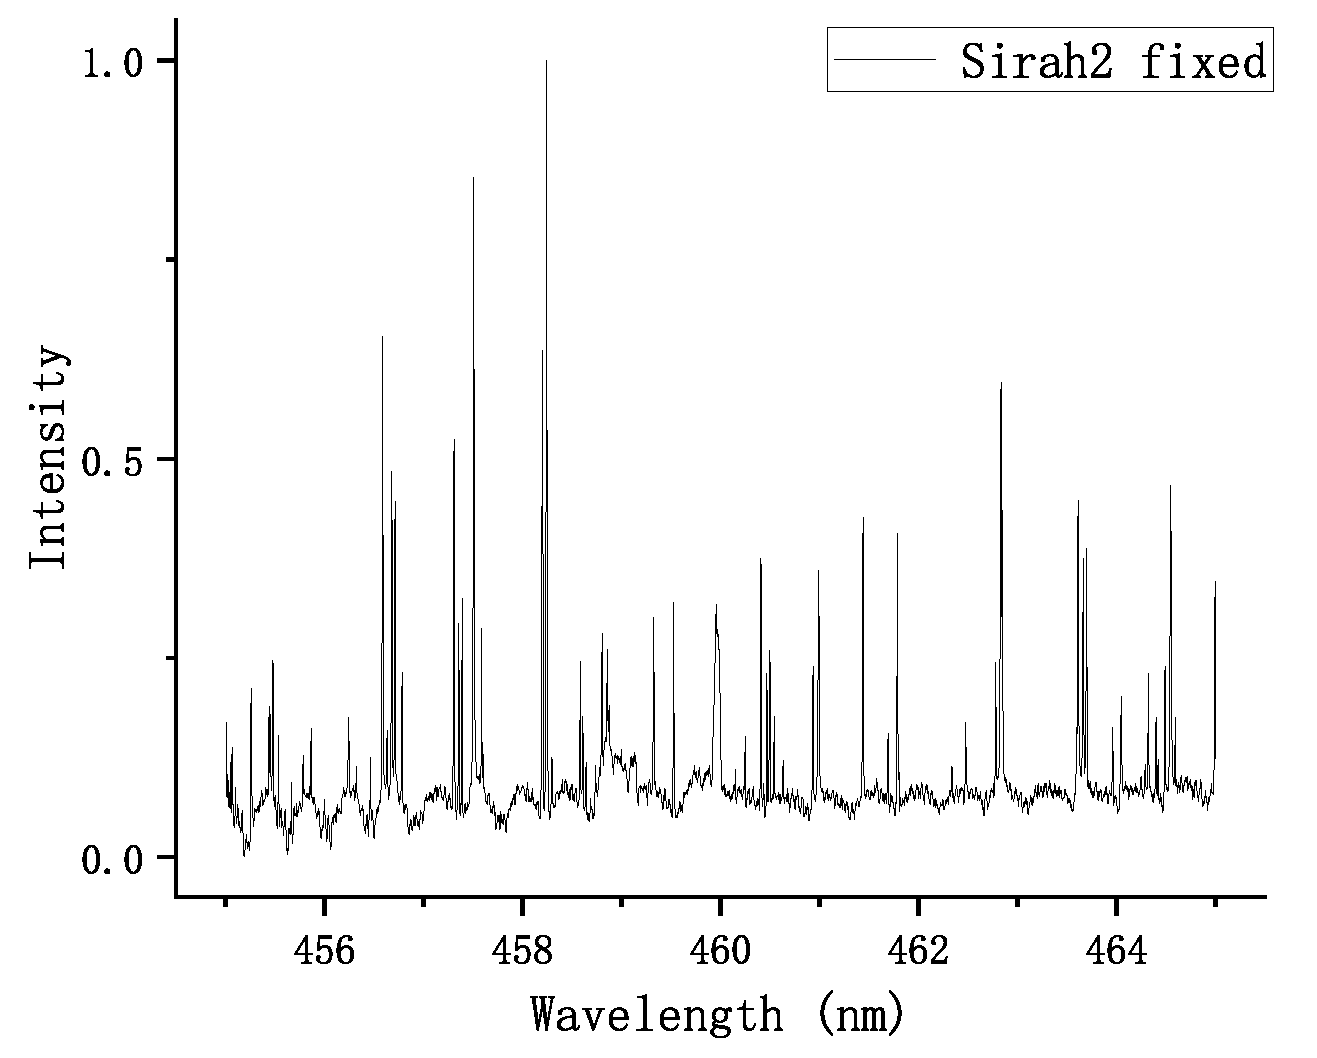
\includegraphics[width=0.6\textwidth]{sirah2fixed.eps}};}
					\onslide<2>{\node at (0,0){\includegraphics[width=0.6\textwidth]{wavelen_corrected.pdf}};}
			\end{tikzpicture}
			\caption{Wavelen. correction}
		\end{figure}
	\end{frame}
	\begin{frame}{\insertsection}{Calibration}
		\begin{figure}[H]
			\centering
			\includegraphics[width=0.6\textwidth]{fitfunc.pdf}
			\caption{Correction function}
		\end{figure}
	\end{frame}
\section{REMPI scan}
\subsection{Selected peaks}
\begin{frame}{\insertsubsection}
\begin{figure}[H]
\centering
\begin{tikzpicture}
			\draw[white] (4.03,-3.65) rectangle (4,3.65);
			\node at (0,0){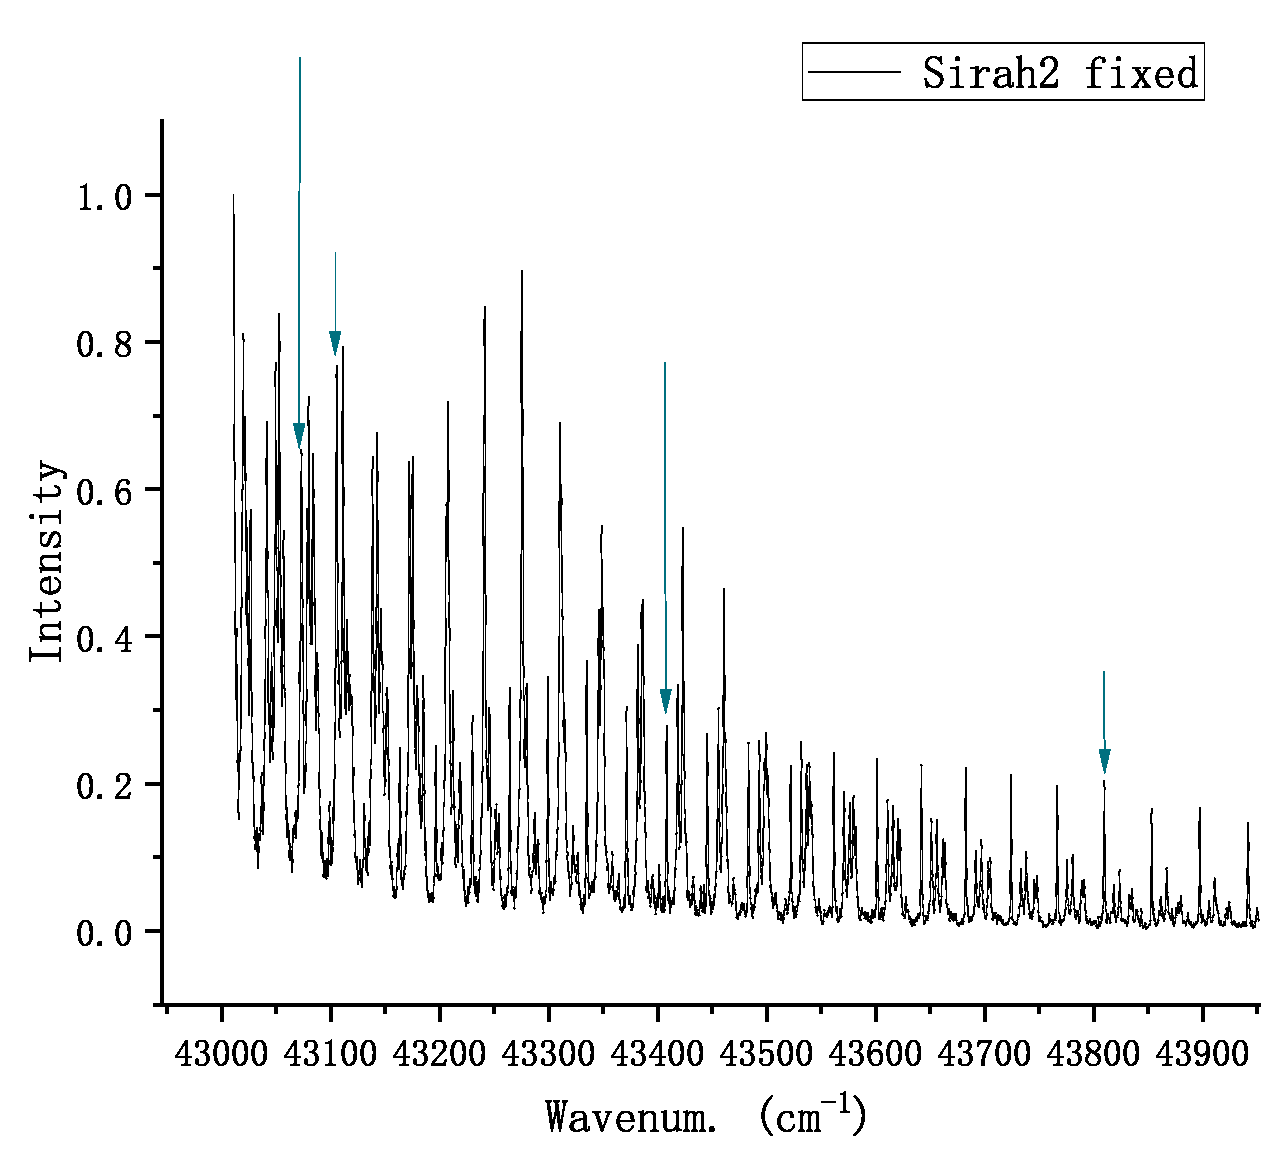
\includegraphics[width=0.6\textwidth]{scanmark.eps}};
			\filldraw[white] (-1.92,2.5) rectangle (-1.88,2.89);
			\node at (-1.5,2.7){\textcolor[RGB]{0,112,127}{$\num{464.484}\unit{\nano \meter}$}};
			\node at (-0.93,2.03){\textcolor[RGB]{0,112,127}{$\num{464.114}\unit{\nano \meter}$}};
			\node at (0.47,1.5){\textcolor[RGB]{0,112,127}{$\num{460.875}\unit{\nano \meter}$}};
			\node at (2.3,-0.25){\textcolor[RGB]{0,112,127}{$\num{456.659}\unit{\nano \meter}$}};
\end{tikzpicture}
\end{figure}
\end{frame}
%\begin{frame}{Contents}
%\tableofcontents[currentsection,currentsubsection]
%\end{frame}
%\subsection{Radius and angular distributions}
\begin{frame}{Peak 1}
	\begin{figure}[H]
		\centering
		\begin{tikzpicture}
	\onslide<1,2>{\node at (0,0){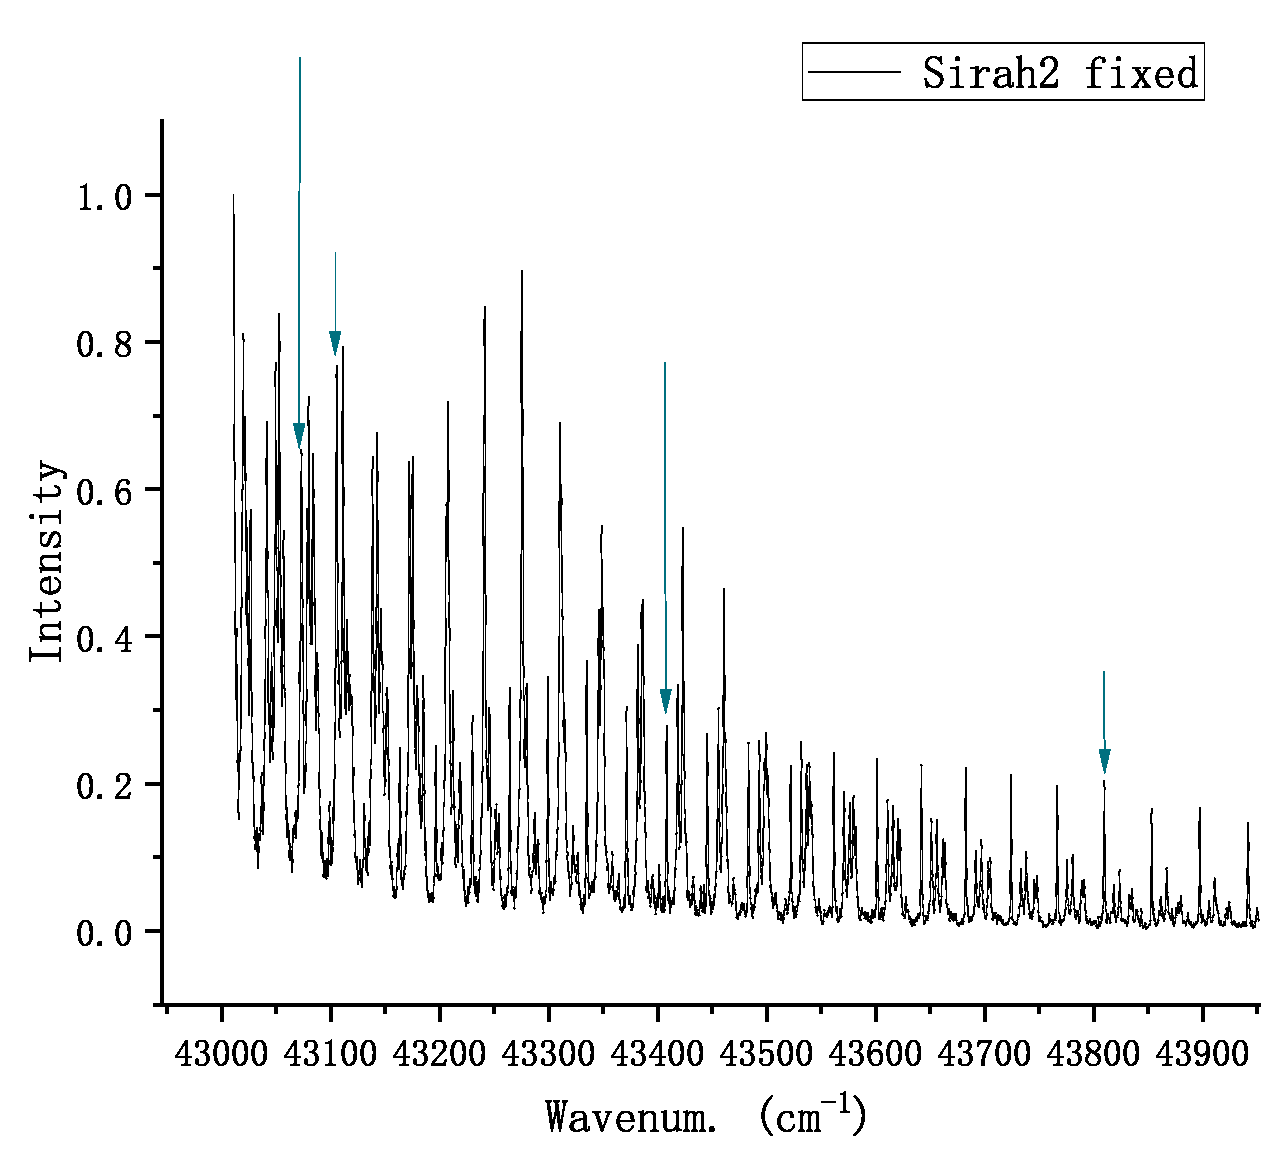
\includegraphics[width=0.6\textwidth]{scanmark.eps}};
	\filldraw[white] (-1.92,2.5) rectangle (-1.88,2.89);
	\node at (-1.5,2.7){\textcolor[RGB]{0,112,127}{$\num{464.484}\unit{\nano \meter}$}};
}
\onslide<2>{
	\node at (2.03,2.4){{\quad\!}rR2(44.5)};
	\node at (2.03,2){\textcolor{red}{{\quad\!}qR12(51.5)}};
	\node at (2.03,1.6){\textcolor{red}{{\quad\!}qQ2(51.5)}};
}
	\onslide<3>{\node at (-1.55,2){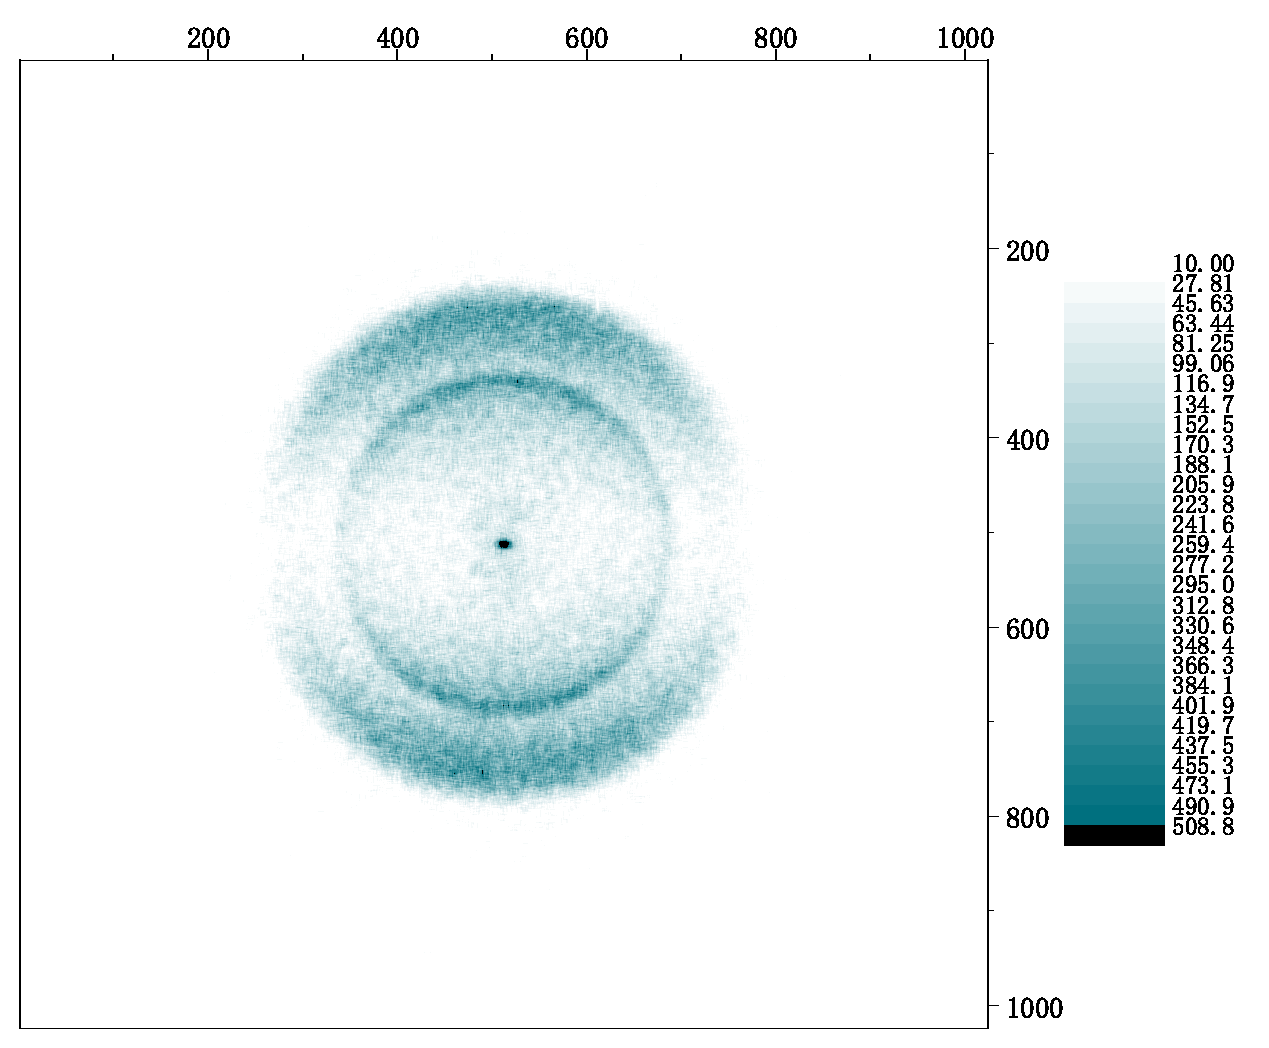
\includegraphics[width = 4cm]{gring_464484.eps}};
	\node at (2.45,2){\includegraphics[width=4cm]{aring_464484.eps}};
	\node at (-2,-2){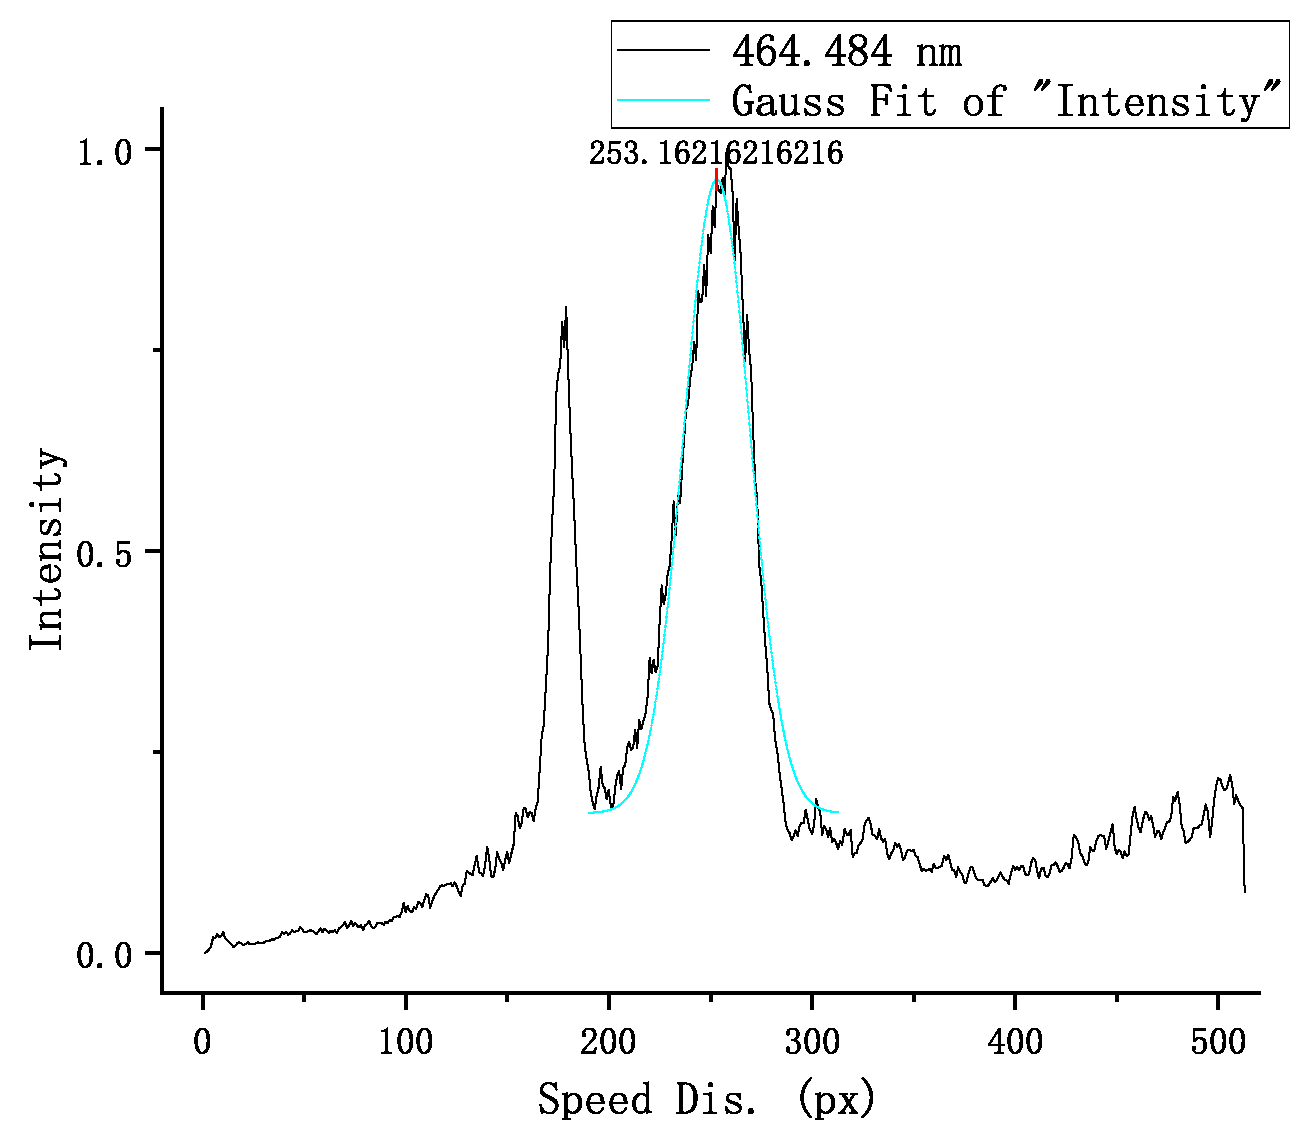
\includegraphics[width=4cm]{rdis_peak_464484.eps}};
	\node at (2,-2){\includegraphics[width=4cm]{adis_464484b.eps}};
	\node at (1.3,-3.2){\textcolor[RGB]{0,112,127}{\small $\beta \approx 1.52$}};
		\node at (-3.0,3.3){\textcolor[RGB]{0,112,127}{smear}};
	\node at (3.07,3.3){\textcolor[RGB]{0,112,127}{Abel${}^{-1}$}};}
\end{tikzpicture}
\end{figure}
\end{frame}
\begin{frame}{Peak 2}
	\begin{figure}[H]
		\centering
		\begin{tikzpicture}
	\onslide<1,2>{\node at (0,0){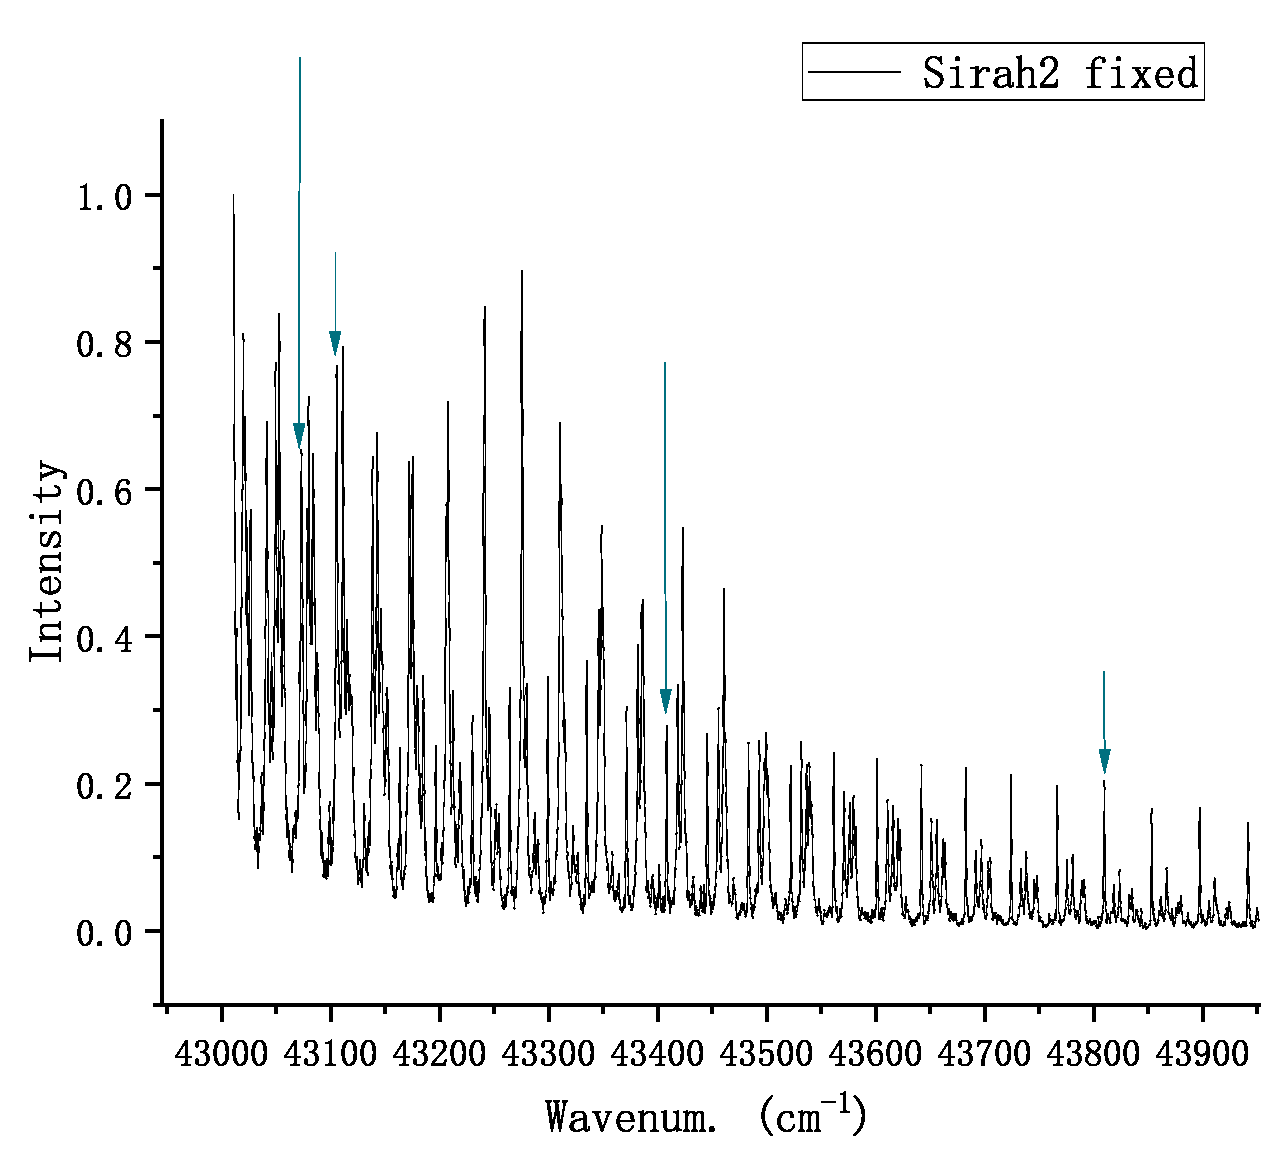
\includegraphics[width=0.6\textwidth]{scanmark.eps}};
	\filldraw[white] (-1.92,2.5) rectangle (-1.88,2.89);
			\node at (-0.93,2.03){\textcolor[RGB]{0,112,127}{$\num{464.114}\unit{\nano \meter}$}};
}
\onslide<2>{	
	\node at (2.03,2.4){{\quad\!}rR2(45.5)};
	\node at (2.03,2){\textcolor{red}{{\quad\!}qR12(51.5)}};
	\node at (2.03,1.6){\textcolor{red}{{\quad\!}qQ2(51.5)}};
}
		\onslide<3>{\node at (-1.55,2){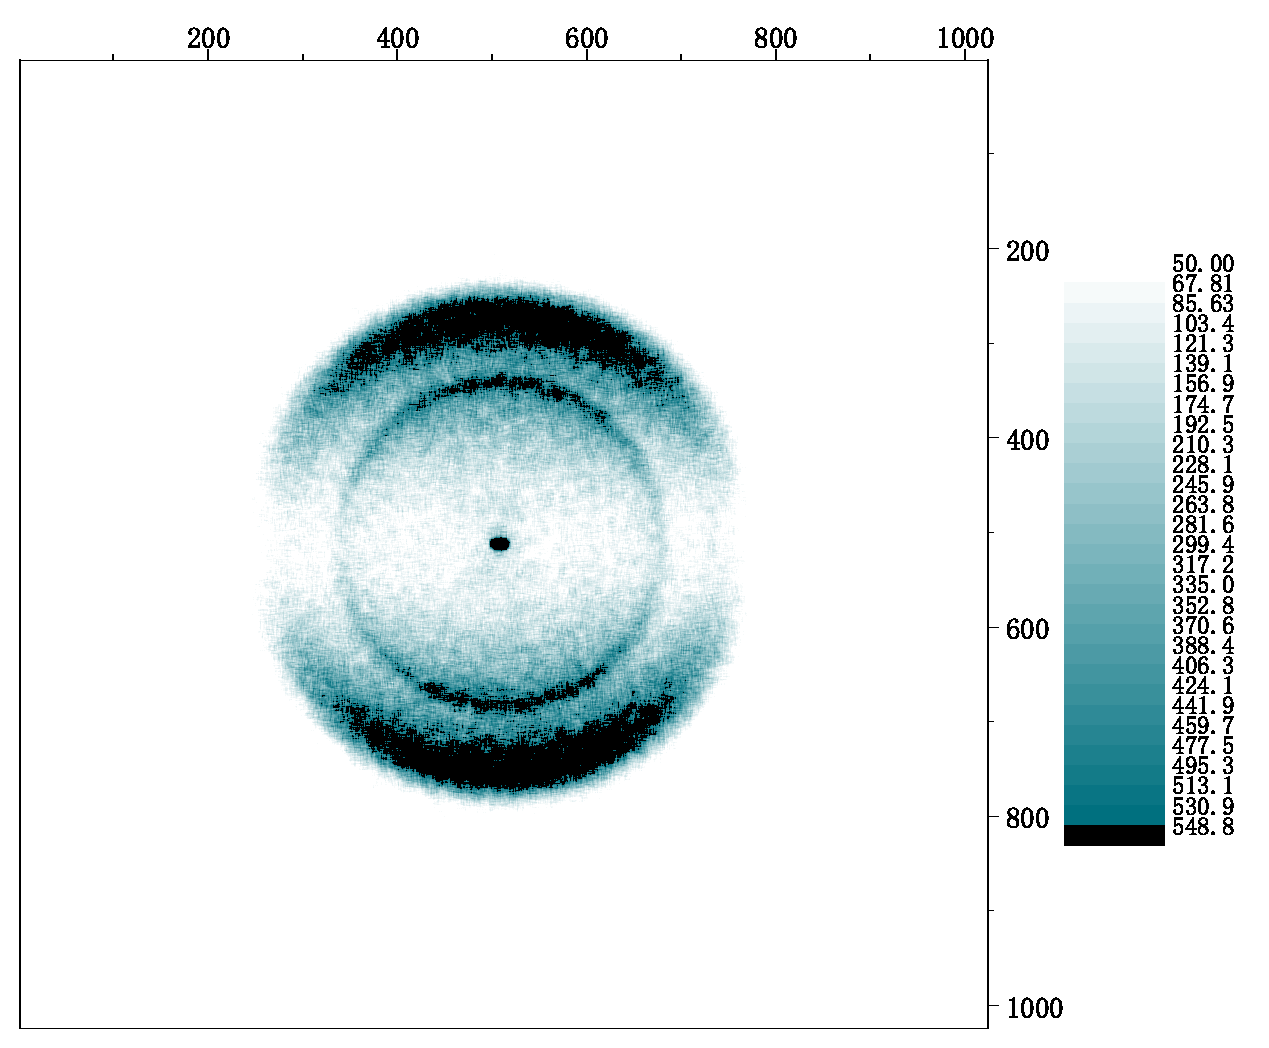
\includegraphics[width = 4cm]{gring_464114.eps}};
			\node at (2.45,2){\includegraphics[width=4cm]{aring_464114.eps}};
			\node at (-2,-2){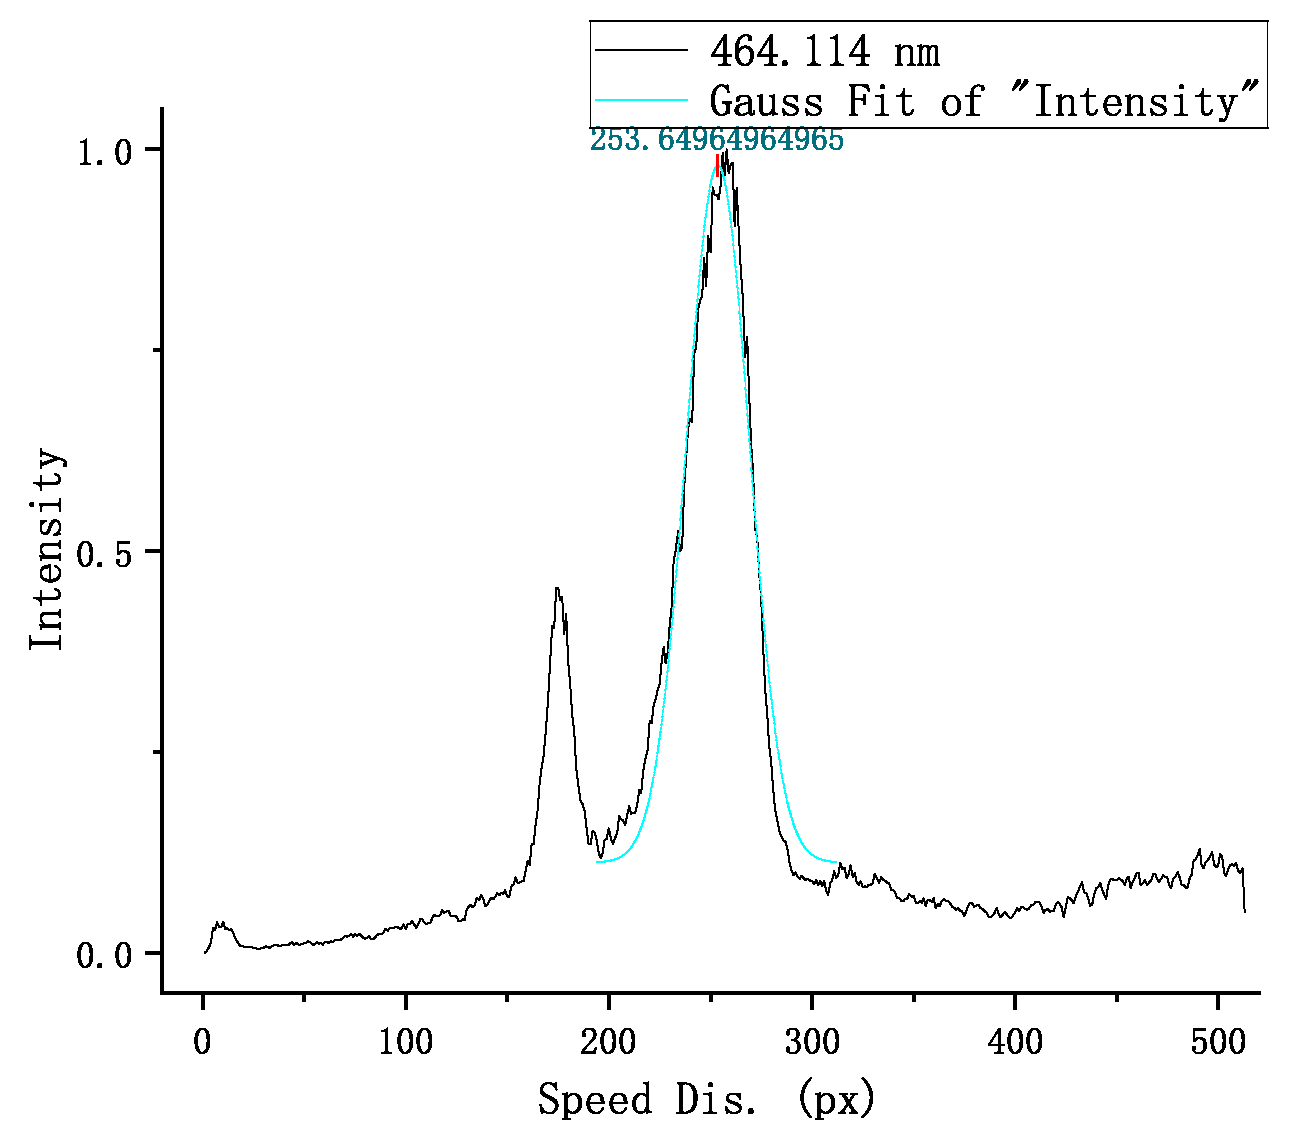
\includegraphics[width=4cm]{rdis_peak_464114.eps}};
			\node at (2,-2){\includegraphics[width=4cm]{adis_464114b.eps}};
			\node at (1.3,-3.2){\textcolor[RGB]{0,112,127}{\small $\beta \approx 1.22$}};
				\node at (-3.0,3.3){\textcolor[RGB]{0,112,127}{smear}};
			\node at (3.07,3.3){\textcolor[RGB]{0,112,127}{Abel${}^{-1}$}};
			}
\end{tikzpicture}
\end{figure}
\end{frame}
\begin{frame}{Peak 3}
\begin{figure}[H]
\centering
\begin{tikzpicture}
			\onslide<1,2>{\node at (0,0){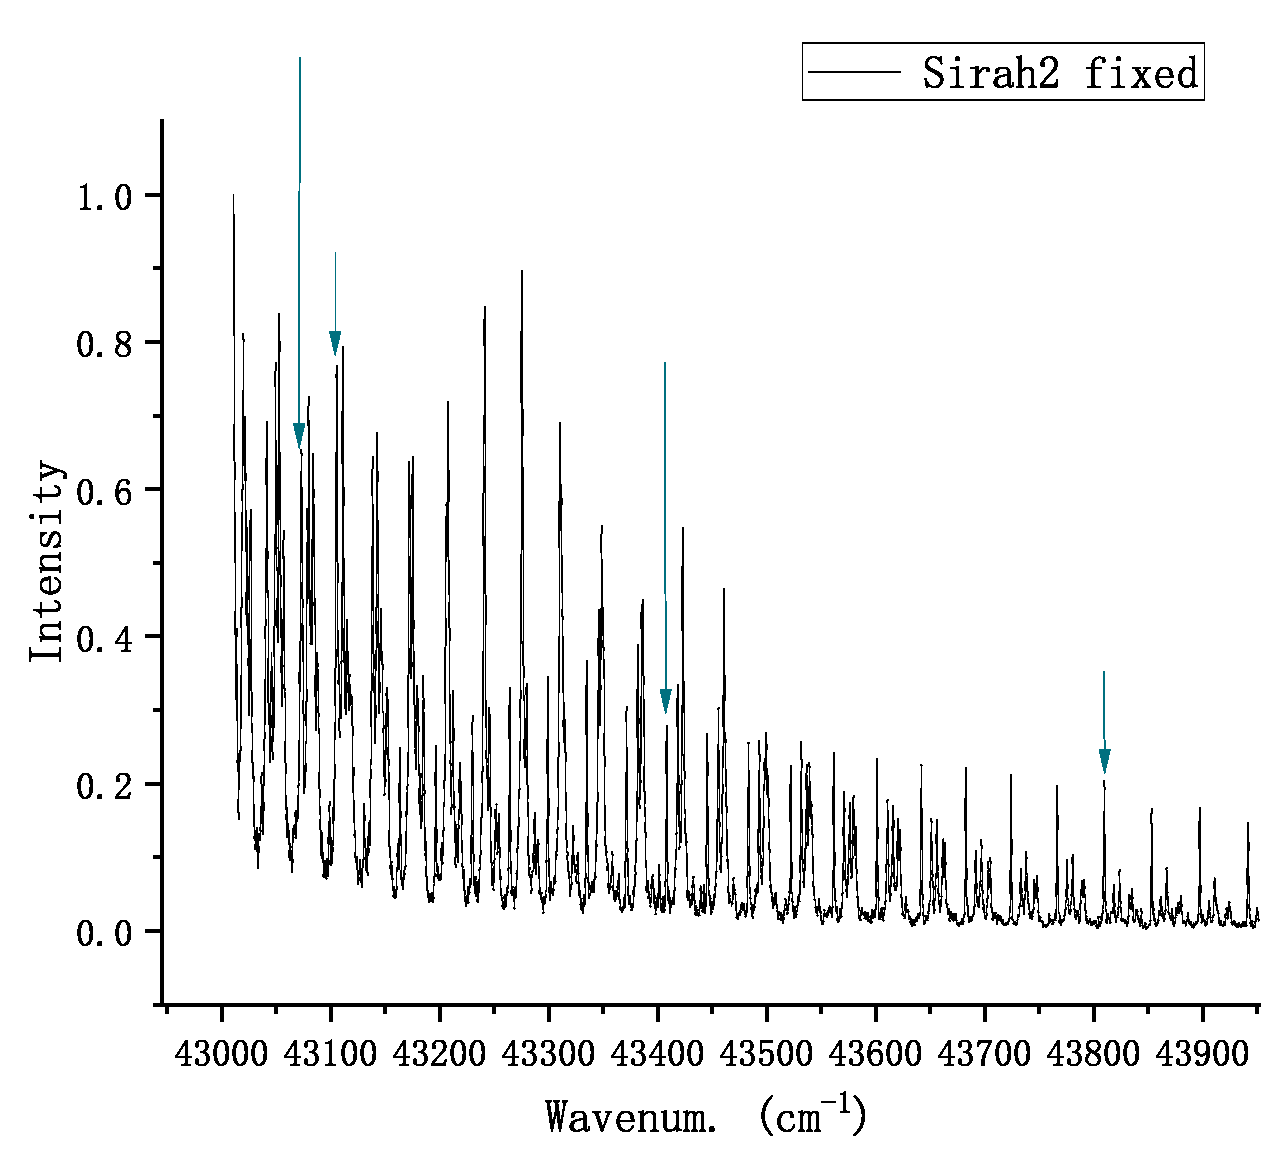
\includegraphics[width=0.6\textwidth]{scanmark.eps}};
			\filldraw[white] (-1.92,2.5) rectangle (-1.88,2.89);
			\node at (0.47,1.5){\textcolor[RGB]{0,112,127}{$\num{460.875}\unit{\nano \meter}$}};
			}
			\onslide<2>{
				\node at (2.03,2.4){{\quad\!}sR21(48.5)};
			}
			\onslide<3>{\node at (-1.55,2){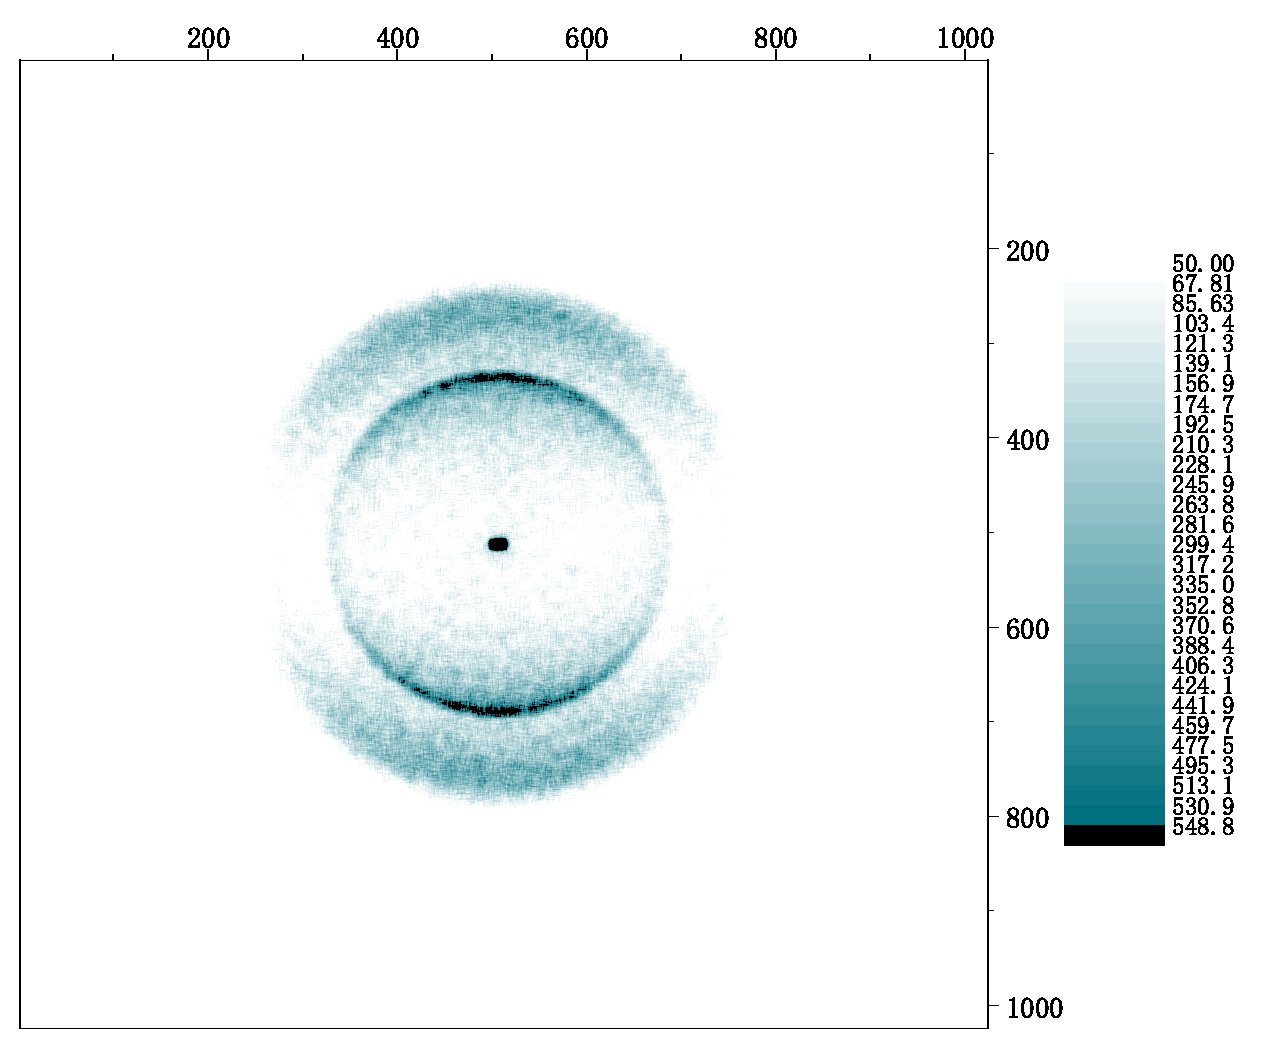
\includegraphics[width = 4cm]{gring460875.eps}};
			\node at (2.45,2){\includegraphics[width=4cm]{aring460875.eps}};
			\node at (-2,-2){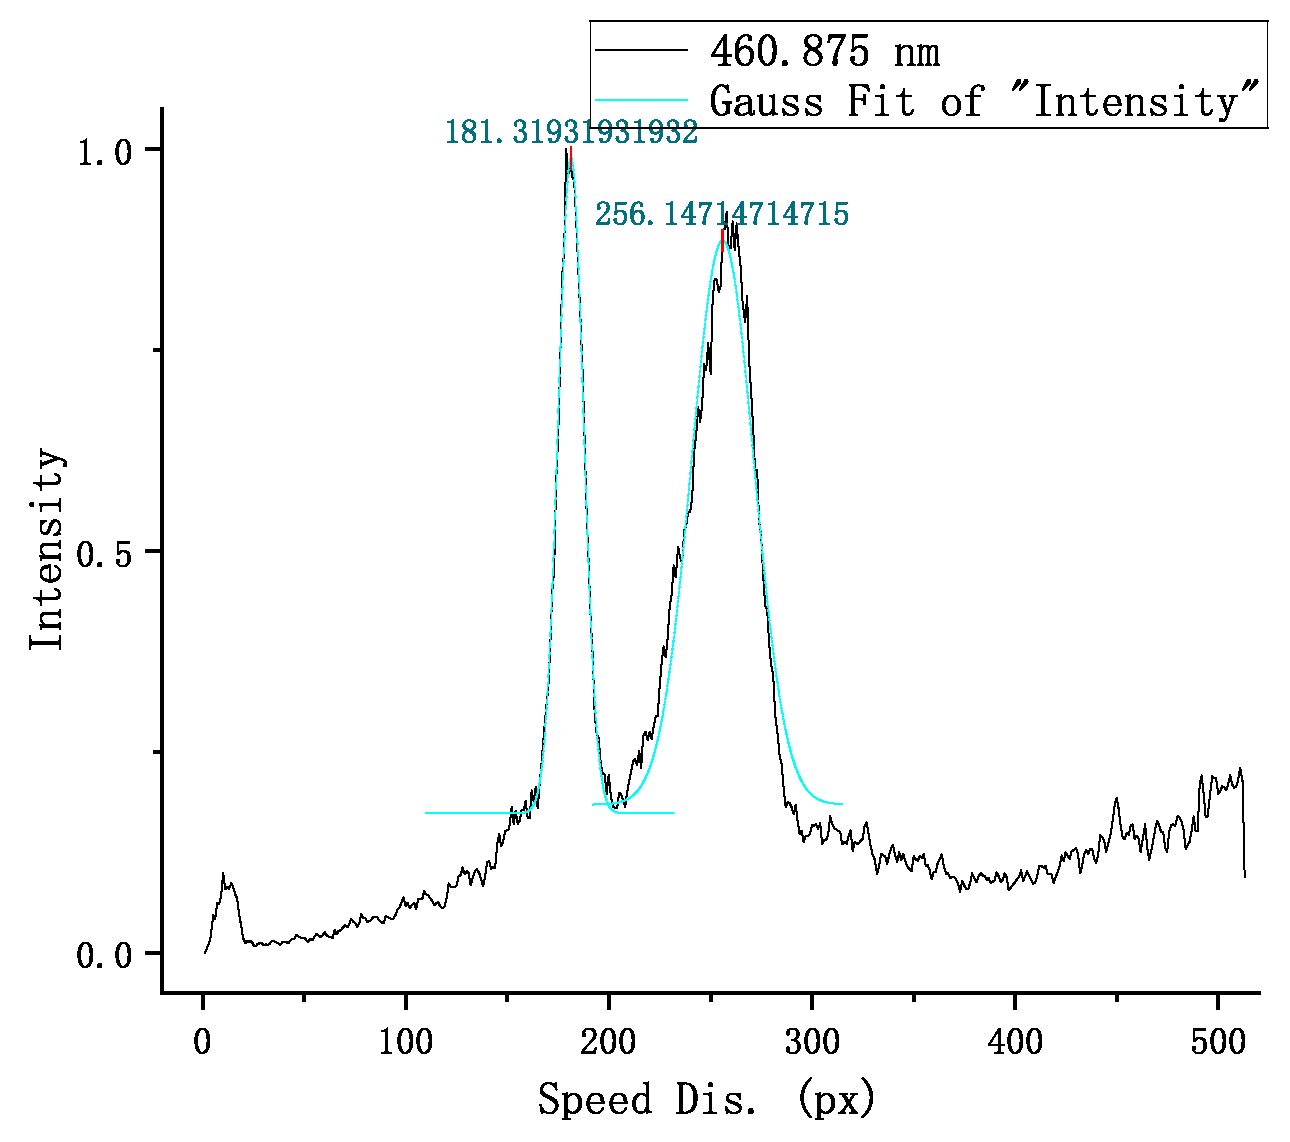
\includegraphics[width=4cm]{rdis_peak_460875.eps}};
			\node at (2,-2){\includegraphics[width=4cm]{adis_460875b.eps}};
			\node at (1.3,-3.2){\textcolor[RGB]{0,112,127}{\small$\beta \approx 0.864$}};
				\node at (-3.0,3.3){\textcolor[RGB]{0,112,127}{smear}};
			\node at (3.07,3.3){\textcolor[RGB]{0,112,127}{Abel${}^{-1}$}};}
\end{tikzpicture}
\end{figure}
\end{frame}
\begin{frame}{Peak 4}
\begin{figure}[H]
\centering
\begin{tikzpicture}
		\onslide<1,2>{
			\node at (0,0){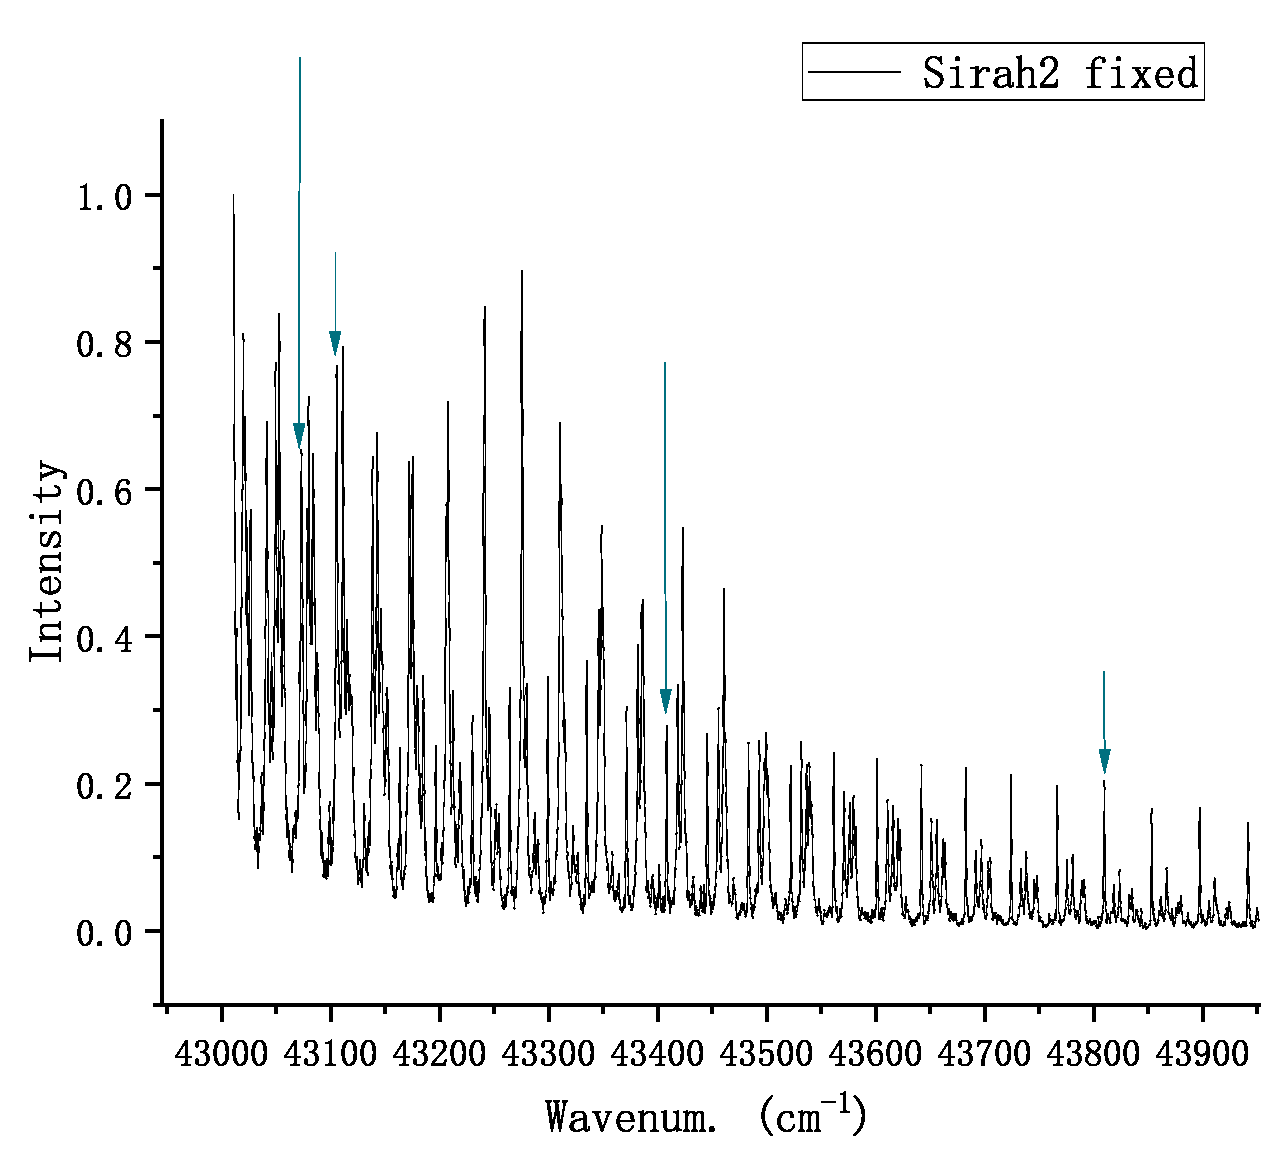
\includegraphics[width=0.6\textwidth]{scanmark.eps}};
			\filldraw[white] (-1.92,2.5) rectangle (-1.88,2.89);
			\node at (2.3,-0.25){\textcolor[RGB]{0,112,127}{$\num{456.659}\unit{\nano \meter}$}};
}
\onslide<2>{
			\node at (2.03,2.4){{\quad\!}sR21(58.5)};
			\node at (2.03,2){\textcolor{red}{{\quad\!}pQ12(76.5)}};
			\node at (2.03,1.6){\textcolor{red}{{\quad\!}pQ2(76.5)}};
}
			\onslide<3>{\node at (-1.55,2){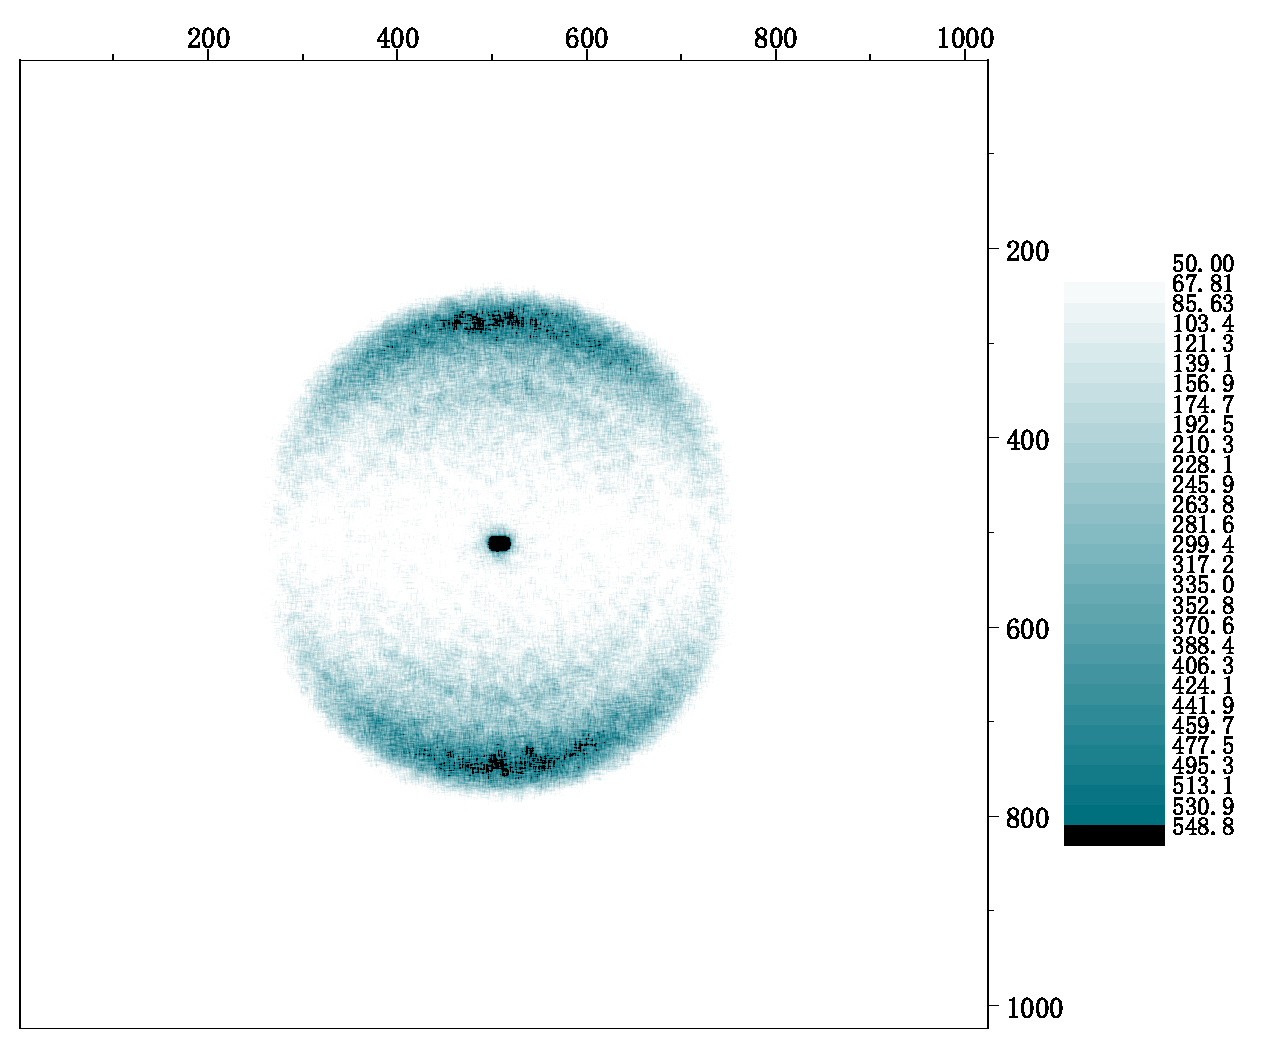
\includegraphics[width = 4cm]{gring456659.eps}};
			\node at (2.45,2){\includegraphics[width=4cm]{aring456659.eps}};
			\node at (-2,-2){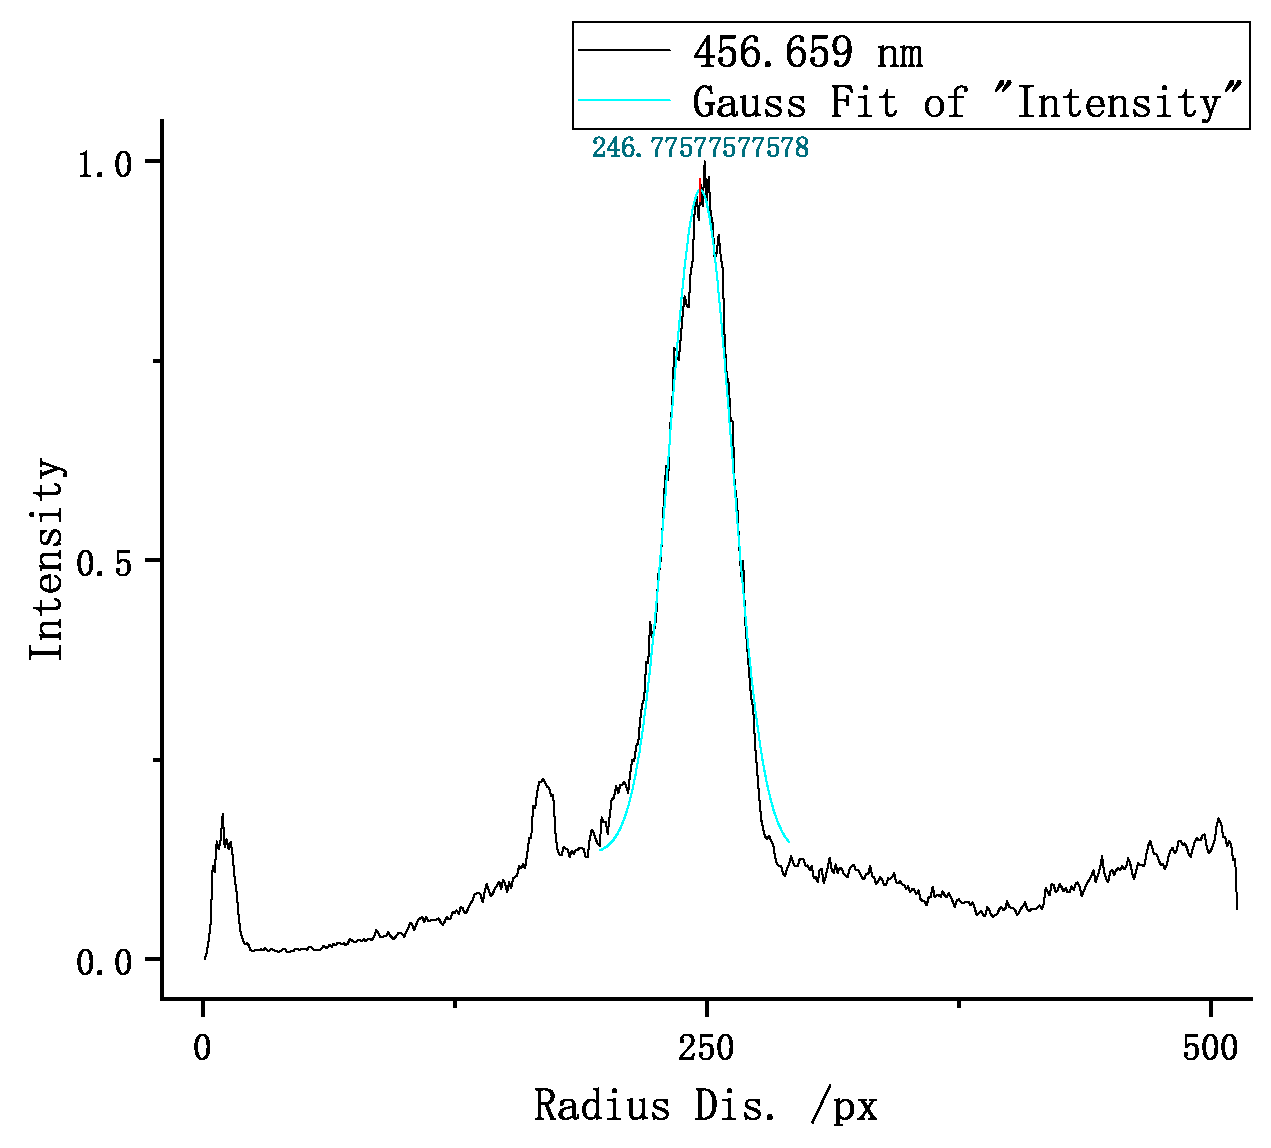
\includegraphics[width=4cm]{rdis_peak_456659.eps}};
			\node at (2,-2){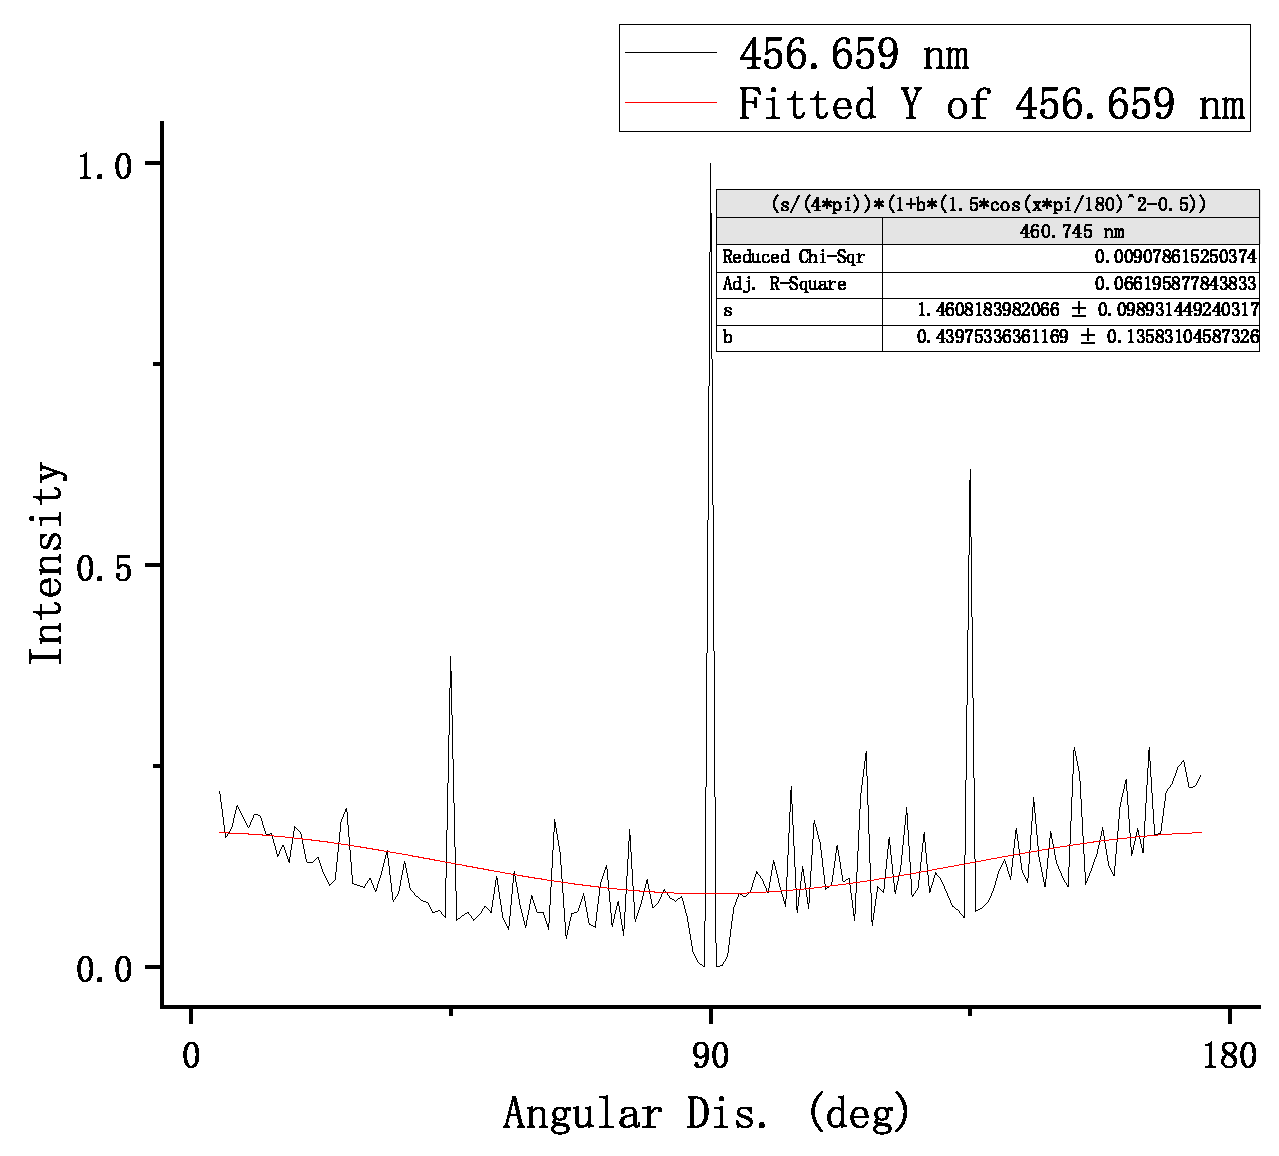
\includegraphics[width=4cm]{adis_456659b.eps}};
			\node at (1.3,-1.2){\small\textcolor[RGB]{0,112,127}{$\beta \approx 0.440$}};
				\node at (-3.0,3.3){\textcolor[RGB]{0,112,127}{smear}};
			\node at (3.07,3.3){\textcolor[RGB]{0,112,127}{Abel${}^{-1}$}};}
\end{tikzpicture}
\end{figure}
\end{frame}
\begin{frame}{Contents}
\tableofcontents[currentsection,currentsubsection]
\end{frame}
\subsection{Peak assignments}
\begin{frame}{\insertsubsection}\nocite{pgopher}
			\begin{table}
			\centering  	 
			\scriptsize
			\begin{tabularx}{0.97\textwidth}{llll}    
				\toprule   
				$464.484 \unit{\nano \meter}$ &$464.114\unit{\nano \meter}$&$460.875 \unit{\nano \meter}$& $456.659 \unit{\nano \meter}$\\
				$\approx43058.49 \unit{\per \centi \meter}$ &   $\approx43092.81\unit{\per \centi \meter}$ &  $\approx 43395.69\unit{\per \centi \meter}$ & $\approx 43796.34\unit{\per \centi \meter} $\\
				\midrule   
				$\text{px}=253.162$ & $\text{px}=253.655$ & $\text{px}=\textcolor{red}{181.319}\,\&\,256.240$ &$ \text{px}=246.776$ \\  
				\midrule 
				$rR2\left( 44.5\right) $ & $rR2\left( 45.5\right) $ &  &$sR21\left( 58.5\right) $\\  
				\textcolor{red}{$qR12\left( 51.5\right) $} & \textcolor{red}{$qR12 \left( 51.5\right) $} &  $sR21\left( 48.5\right) $ & \textcolor{red}{$pQ12 \left( 76.5\right) $} \\ 
				\textcolor{red}{$qQ2\left(  51.5\right) $} & \textcolor{red}{$qQ2\left(  51.5\right) $} &   & \textcolor{red}{$pP2\left(  76.5\right) $} \\ 
				\bottomrule    
			\end{tabularx}%  
			\label{tab:addlabel}%
		\end{table}%
		\begin{alertblock}{Notice}
			\textcolor{red}{Colored} assignments are mismatched, and will not be used to calculate.
		\end{alertblock}
	\end{frame}
	\begin{frame}{Contents}
		\tableofcontents[currentsection,currentsubsection]
	\end{frame}
	\subsection{Speed correction}
		\subsubsection{Trans. energy of \ce{NO}}
	\begin{frame}{\insertsubsection}{\insertsubsubsection}
		\begin{table}[htbp]
			\centering
			\tiny
			\begin{tabularx}{0.9\textwidth}{lccc}
				\toprule
				& $E_\text{total}$ & $E_\text{bond}(\ce{O-NO})$ \footfullcite{ono}& $E_\text{int.}(\ce{NO})$ \\
				\midrule
				Peak 1 & \multirow{2}[2]{*}{$\num{43058.49}\unit{\per \centi \meter}$} & \multirow{8}[8]{*}{$\num{25128.57}\unit{\per \centi \meter}$} & \multirow{2}[2]{*}{\quad\quad\,$\Delta E_v (1\rightarrow 0)+ E( J = 44 )$\quad\quad\,} \\
				$\num{464.484}\unit{\nano\meter}$ & & & \\
				\cmidrule{1-2}\cmidrule{4-4}
				Peak 2 & \multirow{2}[2]{*}{$\num{43092.81}\unit{\per \centi \meter}$} & & \multirow{2}[2]{*}{\quad\quad\,$\Delta E_v (1\rightarrow 0)+ E( J = 45 )$\quad\quad\,} \\
				$\num{464.114}\unit{\nano\meter}$ & & & \\
				\cmidrule{1-2}\cmidrule{4-4}
				Peak 3 & \multirow{2}[2]{*}{$\num{43395.69}\unit{\per \centi \meter}$} & & \multirow{2}[2]{*}{\quad\quad\,$\Delta E_v (1\rightarrow 0)+ E( J = 48 )$\quad\quad\,} \\
				$\num{460.875}\unit{\nano\meter}$ & & & \\
				\cmidrule{1-2}\cmidrule{4-4}
				Peak 4 & \multirow{2}[2]{*}{$\num{43796.34}\unit{\per \centi \meter}$} & & \multirow{2}[2]{*}{\quad\quad\,$\Delta E_v (1\rightarrow 0)+ E( J = 58 )$\quad\quad\,} \\
				$\num{456.659}\unit{\nano\meter}$ & & & \\
				\bottomrule
			\end{tabularx}
		\end{table}
	\end{frame}
	\begin{frame}{\insertsubsection}{\insertsubsubsection}
		\begin{table}[htbp]
			\centering
			\tiny
			\begin{tabularx}{0.9\textwidth}{lccc}
				\toprule
				                                  &                       $E_\text{total}$                        &         $E_\text{bond}(\ce{O-NO})$\footfullcite{ono}          &                            $E_\text{int.}(\ce{NO})$                            \\ \midrule
				Peak 1                            & \multirow{2}[2]{*}{$\num{43058.49}\unit{\per \centi \meter}$} & \multirow{8}[8]{*}{$\num{25128.57}\unit{\per \centi \meter}$} & \multirow{2}[2]{*}{$\num{2341.9327750}\unit{\per \centi \meter}+ E( J = 44 )$} \\
				$\num{464.484}\unit{\nano\meter}$ &                                                               &                                                               &                                                                                \\ \cmidrule{1-2}\cmidrule{4-4}
				Peak 2                            & \multirow{2}[2]{*}{$\num{43092.81}\unit{\per \centi \meter}$} &                                                               & \multirow{2}[2]{*}{$\num{2341.9327750}\unit{\per \centi \meter}+ E( J = 45 )$} \\
				$\num{464.114}\unit{\nano\meter}$ &                                                               &                                                               &                                                                                \\ \cmidrule{1-2}\cmidrule{4-4}
				Peak 3                            & \multirow{2}[2]{*}{$\num{43395.69}\unit{\per \centi \meter}$} &                                                               & \multirow{2}[2]{*}{$\num{2341.9327750}\unit{\per \centi \meter}+ E( J = 48 )$} \\
				$\num{460.875}\unit{\nano\meter}$ &                                                               &                                                               &                                                                                \\ \cmidrule{1-2}\cmidrule{4-4}
				Peak 4                            & \multirow{2}[2]{*}{$\num{43796.34}\unit{\per \centi \meter}$} &                                                               & \multirow{2}[2]{*}{$\num{2341.9327750}\unit{\per \centi \meter}+ E( J = 58 )$} \\
				$\num{456.659}\unit{\nano\meter}$ &                                                               &                                                               &                                                                                \\ \bottomrule
			\end{tabularx}
		\end{table}
		\onslide<2>{\begin{block}{Vib. energy level}
			$E_v  = \omega_e\left( v+\frac{1}{2} \right) -\omega_e x_e\left( v+\frac{1}{2} \right)^2+\omega_e y_e\left( v+\frac{1}{2} \right)^3$.
		\end{block}}
	\end{frame}	
	\begin{frame}{\insertsubsection}{\insertsubsubsection}
		\begin{table}[htbp]
			\centering
			\tiny
			\begin{tabularx}{0.73\textwidth}{lccc}
				\toprule
	 &   $E_\text{total}$  &  $E_\text{bond}(\ce{O-NO})$ \footfullcite{ono}   &  $E_\text{int.}(\ce{NO})$  \\ 
	 \midrule
				Peak 1  & \multirow{2}[2]{*}{$\num{43058.49}\unit{\per \centi \meter}$} & \multirow{8}[8]{*}{$\num{25128.57}\unit{\per \centi \meter}$} & \multirow{2}[2]{*}{\,\;\;$\num{5814.033}\unit{\per \centi \meter}$\,\;\;} \\
				$\num{464.484}\unit{\nano\meter}$ &  &  &\\ \cmidrule{1-2}\cmidrule{4-4}
				Peak 2  & \multirow{2}[2]{*}{$\num{43092.81}\unit{\per \centi \meter}$} &  &  \multirow{2}[2]{*}{$\num{5965.969}\unit{\per \centi \meter}$}       \\
				$\num{464.114}\unit{\nano\meter}$&  &  &    \\ \cmidrule{1-2}\cmidrule{4-4}
				Peak 3  & \multirow{2}[2]{*}{$\num{43395.69}\unit{\per \centi \meter}$} & &  \multirow{2}[2]{*}{$\num{6239.696}\unit{\per \centi \meter}$} \\
				$\num{460.875}\unit{\nano\meter}$ &  &  & \\ \cmidrule{1-2}\cmidrule{4-4}
				Peak 4 & \multirow{2}[2]{*}{$\num{43796.34}\unit{\per \centi \meter}$}&   &  \multirow{2}[2]{*}{$\num{8004.278}\unit{\per \centi \meter}$}\\
				$\num{456.659}\unit{\nano\meter}$ & & & \\
				\bottomrule
			\end{tabularx}
		\end{table}
		\onslide<2>{\begin{block}{Rot. energy level}
			Simulated data generated by PGOPHER\footfullcite{pgopher}.
		\end{block}}
	\end{frame}
	\begin{frame}{\insertsubsection}{\insertsubsubsection}
\begin{table}[htbp]
	\centering
	\tiny
	\begin{tabularx}{0.9\textwidth}{l|cc}
		\toprule
		\multicolumn{1}{l}{\multirow{2}[1]{*}{$E_\text{int.}(\ce{O})$}\footfullcite{3p012}} & \multicolumn{1}{l}{$E_\text{trans} (\text{total})\approx2.875464 E_\text{trans}(\ce{NO}) $} & \multicolumn{1}{l}{$E_\text{trans}(\ce{NO})$} \\
		\multicolumn{1}{l}{} & \multicolumn{1}{l}{$= E_\text{total} -E_\text{bond}(\ce{O-NO})-E_\text{int.}(\ce{O})- E_\text{int.}(\ce{NO}) $} & \multicolumn{1}{l}{ $= \frac{1}{2}m(\ce{NO})v^2(\ce{NO})$} \\
		\midrule
		\multirow{2}[1]{*}{$^3 P_2$} & $11081.356\unit{\per \centi\meter}$ & $4375.588 \unit{\per \centi\meter}$ \\
		& $10964.609\unit{\per \centi\meter}$ & $4334.685 \unit{\per \centi\meter}$ \\
		\multirow{2}[1]{*}{($\num{0}\unit{\per \centi \meter}$)} & $10794.143\unit{\per \centi\meter}$ & $4344.824 \unit{\per \centi\meter}$ \\
		& $9398.766\unit{\per \centi\meter}$ & $3870.489 \unit{\per \centi\meter}$ \\
		\midrule
		\multirow{2}[1]{*}{$^3 P_1$} & $10922.731\unit{\per \centi\meter}$ & $4320.423 \unit{\per \centi\meter}$ \\
		& $10805.984\unit{\per \centi\meter}$ & $4279.520 \unit{\per \centi\meter}$ \\
		\multirow{2}[1]{*}{($\num{158.625}\unit{\per \centi \meter}$)} & $10635.518\unit{\per \centi\meter}$ & $4289.659 \unit{\per \centi\meter}$ \\
		& $9240.141\unit{\per \centi\meter}$ & $3815.324 \unit{\per \centi\meter}$ \\
		\midrule
		\multirow{2}[1]{*}{$^3 P_0$} & $10854.379\unit{\per \centi\meter}$ & $4296.653 \unit{\per \centi\meter}$ \\
		& $10737.632\unit{\per \centi\meter}$ & $4255.749 \unit{\per \centi\meter}$ \\
		\multirow{2}[1]{*}{($\num{226.977}\unit{\per \centi \meter}$)} & $10567.166\unit{\per \centi\meter}$ & $4265.888 \unit{\per \centi\meter}$ \\
		& $9171.789\unit{\per \centi\meter}$ & $3791.553 \unit{\per \centi\meter}$ \\
		\bottomrule
	\end{tabularx}%
\end{table}%
\end{frame}
	\subsubsection{Trans. speed of \ce{NO}}
	\begin{frame}{\insertsubsection}{\insertsubsubsection}
\begin{table}[htbp]  
	\centering  
	\tiny   
	\begin{tabular}{l|cc}    
		\toprule
		\multicolumn{1}{l}{\multirow{2}[1]{*}{$E_\text{int.}(\ce{O})$}} & \multicolumn{1}{l}{$v(\ce{NO}) $} & \multirow{2}[1]{*}{$\Delta y $} \\    
		\multicolumn{1}{l}{} & \multicolumn{1}{l}{$= \sqrt {  \frac{2E_\text{trans}(\ce{NO})}{m(\ce{NO})}   }$} &  \\    
		\midrule
		\multirow{2}[1]{*}{$^3 P_2$} & $1867.845 \unit{\meter \per \second}$ & $253.177$ \\          
		& $1859.094 \unit{\meter \per \second}$ & $253.650$ \\    
		\multirow{2}[1]{*}{($\num{0}\unit{\per \centi \meter}$)} & $1861.267 \unit{\meter \per \second}$ & $256.147$ \\          
		& $1756.732 \unit{\meter \per \second}$ & $246.776$ \\    
		\midrule    
		\multirow{2}[1]{*}{$^3 P_1$} & $1856.033 \unit{\meter \per \second}$ & $253.177$ \\          
		& $1847.226 \unit{\meter \per \second}$ & $253.650$ \\    
		\multirow{2}[1]{*}{($\num{158.625}\unit{\per \centi \meter}$)} & $1849.413 \unit{\meter \per \second}$ & $256.148$ \\          
		& $1744.168 \unit{\meter \per \second}$ & $246.776$ \\    
		\midrule    
		\multirow{2}[1]{*}{$^3 P_0$} & $1850.920 \unit{\meter \per \second}$ & $253.177$ \\          
		& $1842.089 \unit{\meter \per \second}$ & $253.650$ \\    
		\multirow{2}[1]{*}{($\num{226.977}\unit{\per \centi \meter}$)} & $1844.282 \unit{\meter \per \second}$ & $256.147$ \\          
		& $1738.726 \unit{\meter \per \second}$ & $246.776$ \\    		
		\bottomrule    
		\end{tabular}
	\end{table}%
\end{frame}
	\begin{frame}{\insertsubsection}{\insertsubsubsection}
		\begin{figure}[H]
			\centering
\begin{tikzpicture}
	\node at (0,0){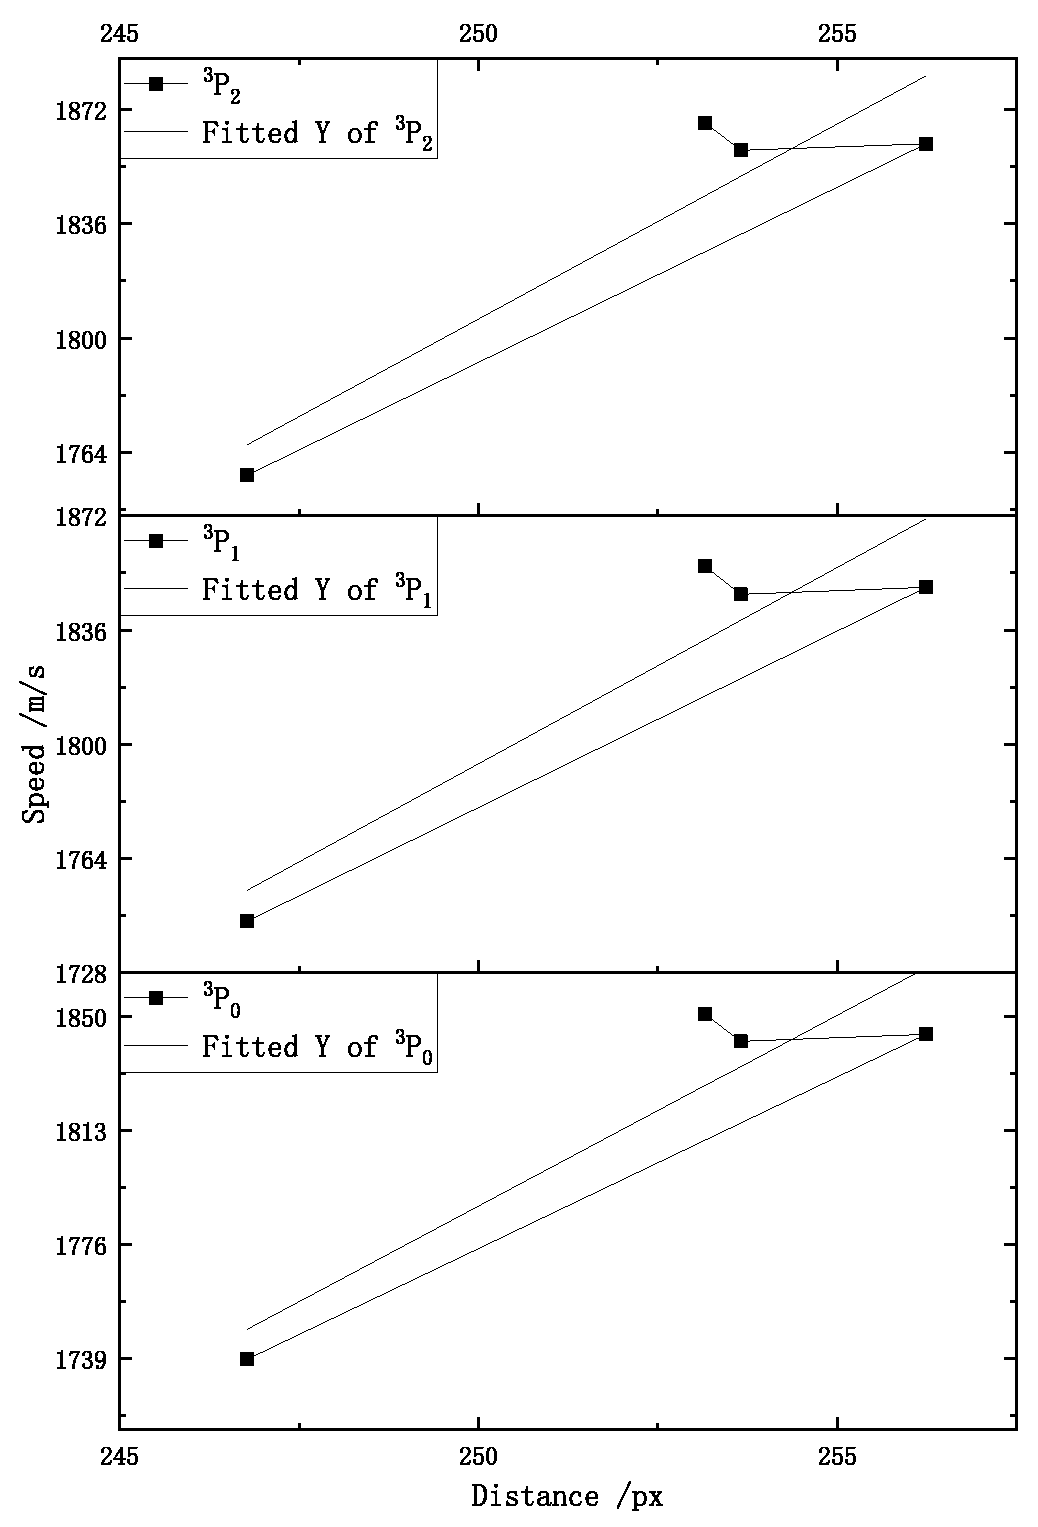
\includegraphics[height=6.8cm]{3p012.eps}};
	\node[anchor=west] at (2.3,2.5){$^3P_2 $};
	\node[anchor=west] at (2.3,2){ $12.28\unit{\meter \per \second }\,\mathrm{px}^{-1} $};
	\node[anchor=west] at (2.3,1.5){Intercept $\approx\num{-1265}\unit{\meter \per \second}$};
	\node[anchor=west] at (2.3,0.5){$^3P_1 $};
	\node[anchor=west] at (2.3,0){$ 12.37\unit{\meter \per \second}\,\mathrm{px}^{-1}$};
	\node[anchor=west] at (2.3,-0.5){Intercept $\approx\num{-1298}\unit{\meter \per \second}$};
	\node[anchor=west] at (2.3,-1.5){$^3P_0 $};
	\node[anchor=west] at (2.3,-2){$ 12.40\unit{\meter \per \second}\,\mathrm{px}^{-1}$};
	\node[anchor=west] at (2.3,-2.5){Intercept $\approx\num{-1313}\unit{\meter \per \second}$};
\end{tikzpicture}
\end{figure}
\end{frame}
\begin{frame}{\insertsubsection}{\insertsubsubsection}
	\begin{figure}[H]
		\centering
\begin{tikzpicture}
	\node at (0,0){\includegraphics[width = 0.6\textwidth]{averagespeed.eps}};
	\node[anchor=west] at (4,0){Average};
	\node[anchor=west] at (4,-0.5){$ 12.35\unit{\meter \per \second}\,\mathrm{px}^{-1}$};
	\node[anchor=west] at (4,-1){Intercept $\approx\num{-1292}\unit{\meter \per \second}$};	
\end{tikzpicture}
		\end{figure}
	\end{frame}
		\begin{frame}{Contents}
		\tableofcontents[currentsection,currentsubsection]
	\end{frame}
	\subsection{Error}
	\begin{frame}{\insertsubsection}
		\begin{figure}[H]
			\centering
			\begin{tikzpicture}
				\node at (0,0){\includegraphics[width = 0.6\textwidth]{averagespeed.eps}};
				\node[anchor=west] at (4,0){Average};
				\node[anchor=west] at (4,-0.5){$ 12.35\unit{\meter \per \second}\,\mathrm{px}^{-1}$};
				\node[anchor=west] at (4,-1){Intercept $\approx\textcolor{red}{\num{-1292}}\unit{\meter \per \second}$};	
			\end{tikzpicture}
		\end{figure}
	\end{frame}
\begin{frame}{\insertsubsection}{\insertsubsubsection}
	\begin{columns}
			\begin{column}{0.45\textwidth}
\begin{tikzpicture}
	\node at (0,0){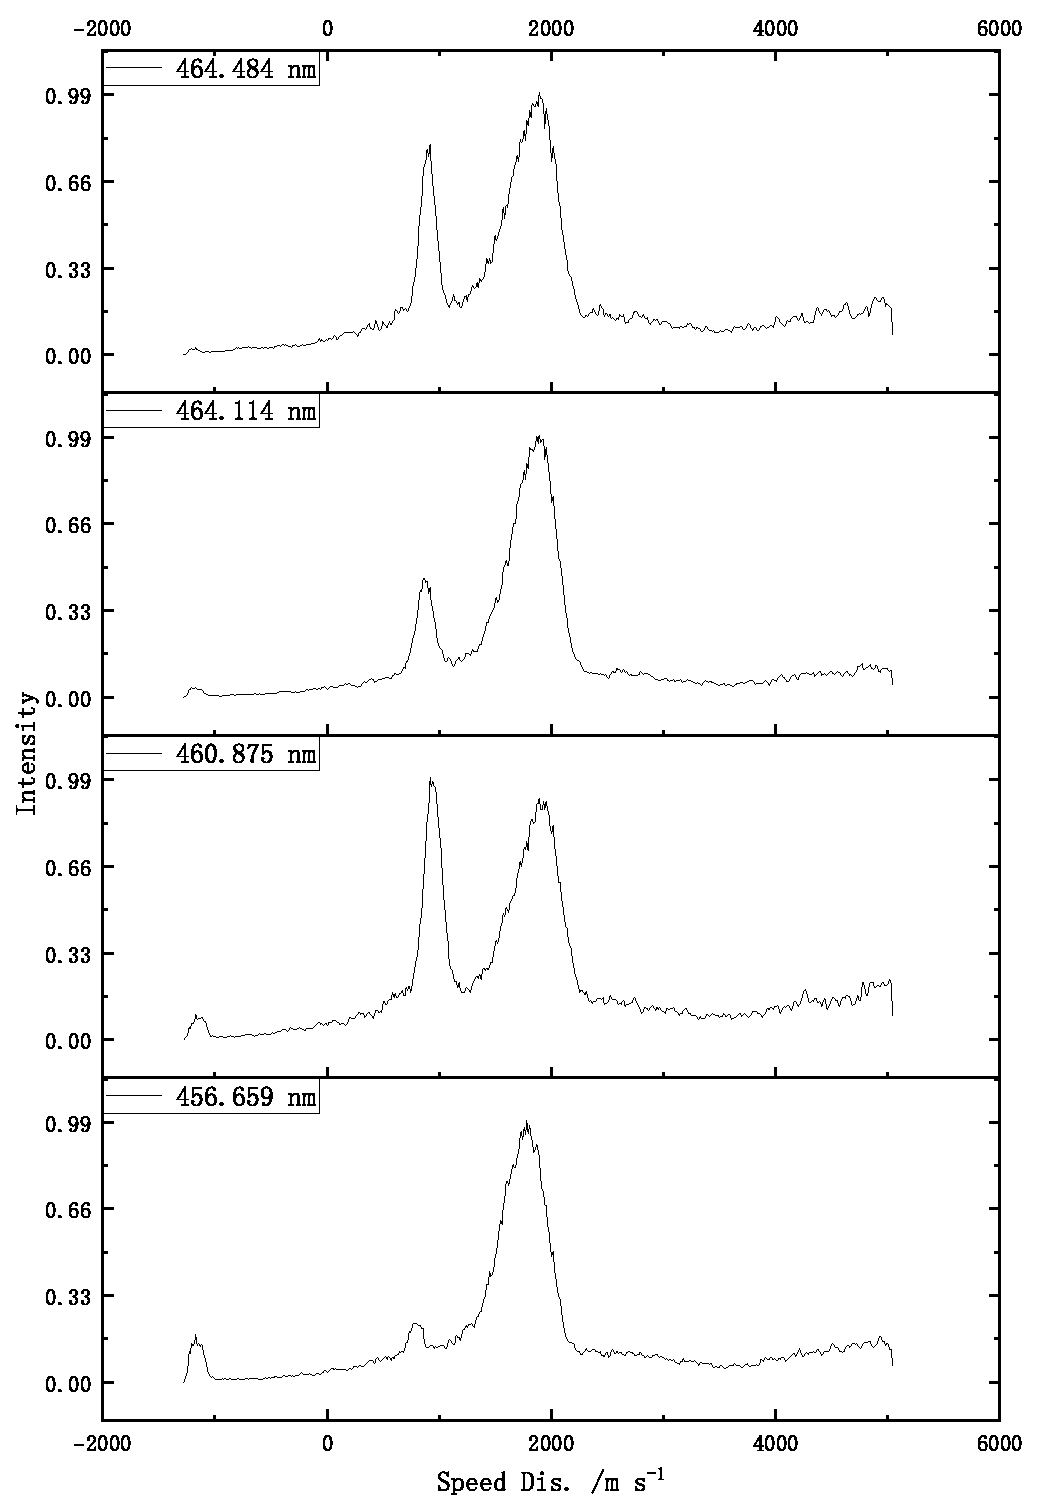
\includegraphics[height=8cm]{vdis.eps}};
	\onslide<2->{
	\draw[trigon,thick] (-1.03,2.06) rectangle (-1.87,2.43);
	\draw[trigon,thick] (-1.03,0.19) rectangle (-1.87,0.56);
	\draw[trigon,thick] (-1.03,-1.68) rectangle (-1.87,-1.31);
	\draw[trigon,thick] (-1.03,-3.54) rectangle (-1.87,-3.17);}
\end{tikzpicture}
				\end{column}
			\begin{column}{0.55\textwidth}
				\onslide<2->{
					Average\\$ 12.35\unit{\meter \per \second}\,\mathrm{px}^{-1}$\\Intercept $\approx\textcolor{red}{\num{-1292}}\unit{\meter \per \second}$	
			}
				\onslide<3->{
					\begin{alertblock}{Notice}
					What we are calculating here are actually $\left| \mathbf{v}_{\ce{NO}}  \right| $, which are not supposed to be  \textcolor{red}{minus}
				\footnote{Maybe a $\num{\pm 5}\unit{\meter \per \second}$-level intercept noise are permitted.}.
				\end{alertblock}
			}
				\end{column}
		\end{columns}
\end{frame}
%	
%	
	\begin{frame}{\insertsubsection}
	\begin{figure}[H]
		\centering
		\begin{tikzpicture}
			\node at (0,0){\includegraphics[width = 0.6\textwidth]{averagespeed.eps}};
			\draw [trigon,rotate=135,anchor=center] (0.5,-2.7) ellipse [x radius=0.5cm, y radius=0.2cm];
			\draw [trigon,rotate=45,anchor=center] (4.7,-0.7) ellipse [x radius=0.5cm, y radius=0.2cm];
			\draw [->] (3.57,2.9) arc(45,135,3);
		\end{tikzpicture}
	\end{figure}
\end{frame}
%	\begin{columns}
	%		\begin{column}{0.65\textwidth}
		%	
		%		\end{column}
	%		\vrule
	%		\begin{column}{0.35\textwidth}
		%			
		%		\end{column}
	%	\end{columns}
%	
%	
%	
%	
%
\section*{Reference}
\begin{frame}{\insertsection}
	\printbibliography
\end{frame}
%	\begin{frame}{Open source}
%このスライドはソースコードが\qrcode[hyperlink,height=2cm]{https://github.com/xiaoyuleiba/MachinetimeReport}にて公開される。
%\end{frame}
\end{document}









